\documentclass{article}
\usepackage[margin=1in]{geometry}
\usepackage{amsmath,amsthm,amssymb}
\usepackage{bbm,enumerate,mathtools}
\usepackage{tikz,pgfplots}
\usepackage{chessboard}
\usepackage[hidelinks]{hyperref}
\usepackage{multicol} % Problem 35
\usepackage{xstring} % Difficulty command
\usetikzlibrary{shapes.geometric}

\newenvironment{question}{\begin{trivlist}\item[\textbf{Question.}]}{\end{trivlist}}
\newenvironment{note}{\begin{trivlist}\item[\textbf{Note.}]}{\end{trivlist}}
\newenvironment{references}{\begin{trivlist}\item[\textbf{References.}]}{\end{trivlist}}
\newenvironment{related}{\begin{trivlist}\item[\textbf{Related.}]\end{trivlist}\begin{enumerate}}{\end{enumerate}}

\newcommand\score[1]{
\pgfmathsetmacro\pgfxa{#1+1}
\tikzstyle{scorestars}=[
  star,
  star points=5,
  star point ratio=2.25,
  draw,
  inner sep=3pt,
  anchor=outer point 5
]
  \begin{tikzpicture}[baseline]
    \draw[opacity=0] (0,-0.5) rectangle (0,0.2); % Workaround for whitespace at the bottom.
    \foreach \i in {1,...,4} {
      \pgfmathparse{(\i<=#1?"yellow":"gray")}
      \edef\starcolor{\pgfmathresult}
      \draw (\i*4.5ex,0) node[name=star\i,scorestars,fill=\starcolor]  {};
    }
  \end{tikzpicture}
}

\newcommand{\difficulty}[1]{%
  \IfEqCase{#1}{%
      {1}{
        
\begin{tikzpicture}[scale=0.7, baseline=0.9mm]%
          \definecolor{slopegreen}{rgb}{0.0, 0.5, 0.0}%
          \fill[slopegreen] (0.5,0.5) circle (0.5);%
        \end{tikzpicture}%
      }%
      {2}{
        
\begin{tikzpicture}[scale=0.7, baseline=0.9mm]%
          \definecolor{slopeblue}{rgb}{0.0, 0.44, 1.00}
          \fill[slopeblue] (0,0) rectangle (1,1);%
        \end{tikzpicture}%
      }%
      {3}{
\begin{tikzpicture}[scale=0.7, baseline=0.9mm]\fill (0,0.5)--(0.5, 0)--(1,0.5)--(0.5,1)--cycle; \end{tikzpicture}}%
      {4}{
\begin{tikzpicture}[scale=0.7, baseline=0.9mm]\fill (0.25,0)--(0,0.5)--(0.25,1)--(0.5,0.5)--cycle; \fill (0.75,0)--(0.5,0.5)--(0.75,1)--(1,0.5)--cycle;\end{tikzpicture}}%
      % you can add more cases here as desired
  }[\PackageError{difficulty}{Undefined difficulty level: #1}{}]%
}%
\newcommand{\rating}[2]{\difficulty{#1}\\\score{#2}\\}


\begin{document}
\rating{3}{4}
From Alec Jones. Let $a_k(n)$ count the number of $k$-gons with vertices on the $n \times n$
grid.
\begin{figure}[!h]
  \centering
  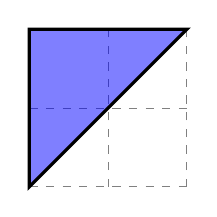
\begin{tikzpicture}
    \draw[gray, dashed] (0,0) grid (2,2);
    \draw[very thick, fill={blue}, fill opacity=0.5] (0,0)--(2,2)--(0,2)--cycle;
  \end{tikzpicture}
  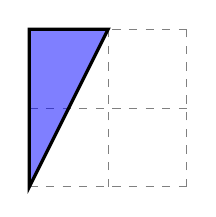
\begin{tikzpicture}
    \draw[gray, dashed] (0,0) grid (2,2);
    \draw[very thick, fill={blue}, fill opacity=0.5] (0,0)--(1,2)--(0,2)--cycle;
  \end{tikzpicture}
  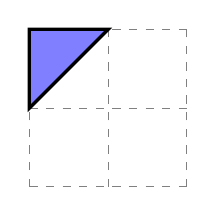
\begin{tikzpicture}
    \draw[gray, dashed] (0,0) grid (2,2);
    \draw[very thick, fill={blue}, fill opacity=0.5] (0,1)--(1,2)--(0,2)--cycle;
  \end{tikzpicture}
  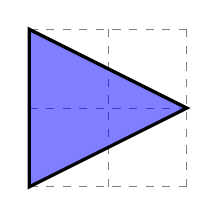
\begin{tikzpicture}
    \draw[gray, dashed] (0,0) grid (2,2);
    \draw[very thick, fill={blue}, fill opacity=0.5] (0,0)--(0,2)--(2,1)--cycle;
  \end{tikzpicture}\\~\\
  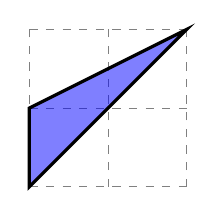
\begin{tikzpicture}
    \draw[gray, dashed] (0,0) grid (2,2);
    \draw[very thick, fill={blue}, fill opacity=0.5] (0,0)--(0,1)--(2,2)--cycle;
  \end{tikzpicture}
  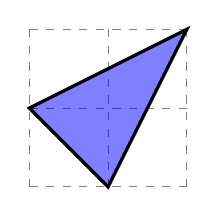
\begin{tikzpicture}
    \draw[gray, dashed] (0,0) grid (2,2);
    \draw[very thick, fill={blue}, fill opacity=0.5] (0,1)--(1,0)--(2,2)--cycle;
  \end{tikzpicture}
  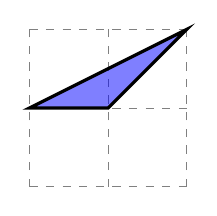
\begin{tikzpicture}
    \draw[gray, dashed] (0,0) grid (2,2);
    \draw[very thick, fill={blue}, fill opacity=0.5] (0,1)--(1,1)--(2,2)--cycle;
  \end{tikzpicture}
  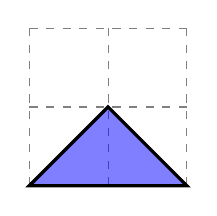
\begin{tikzpicture}
    \draw[gray, dashed] (0,0) grid (2,2);
    \draw[very thick, fill={blue}, fill opacity=0.5] (0,0)--(1,1)--(2,0)--cycle;
  \end{tikzpicture}\\~\\~\\
  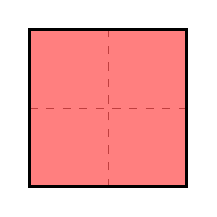
\begin{tikzpicture}
    \draw[gray, dashed] (0,0) grid (2,2);
    \draw[very thick, fill={red}, fill opacity=0.5] (0,0)--(0,2)--(2,2)--(2,0)--cycle;
  \end{tikzpicture}
  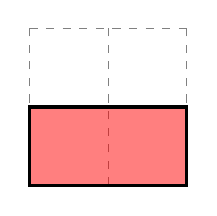
\begin{tikzpicture}
    \draw[gray, dashed] (0,0) grid (2,2);
    \draw[very thick, fill={red}, fill opacity=0.5] (0,0)--(0,1)--(2,1)--(2,0)--cycle;
  \end{tikzpicture}
  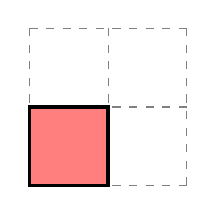
\begin{tikzpicture}
    \draw[gray, dashed] (0,0) grid (2,2);
    \draw[very thick, fill={red}, fill opacity=0.5] (0,0)--(0,1)--(1,1)--(1,0)--cycle;
  \end{tikzpicture}
  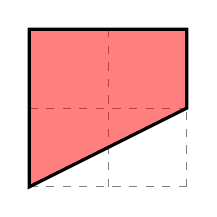
\begin{tikzpicture}
    \draw[gray, dashed] (0,0) grid (2,2);
    \draw[very thick, fill={red}, fill opacity=0.5] (0,0)--(0,2)--(2,2)--(2,1)--cycle;
  \end{tikzpicture}
  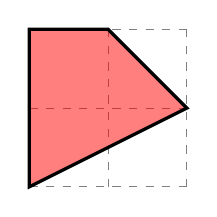
\begin{tikzpicture}
    \draw[gray, dashed] (0,0) grid (2,2);
    \draw[very thick, fill={red}, fill opacity=0.5] (0,0)--(0,2)--(1,2)--(2,1)--cycle;
  \end{tikzpicture}
  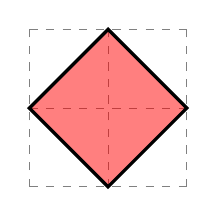
\begin{tikzpicture}
    \draw[gray, dashed] (0,0) grid (2,2);
    \draw[very thick, fill={red}, fill opacity=0.5] (0,1)--(1,0)--(2,1)--(1,2)--cycle;
  \end{tikzpicture}
  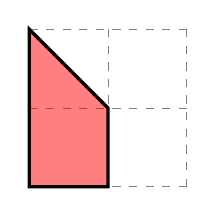
\begin{tikzpicture}
    \draw[gray, dashed] (0,0) grid (2,2);
    \draw[very thick, fill={red}, fill opacity=0.5] (0,0)--(0,2)--(1,1)--(1,0)--cycle;
  \end{tikzpicture}\\~\\
  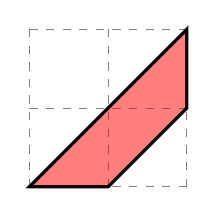
\begin{tikzpicture}
    \draw[gray, dashed] (0,0) grid (2,2);
    \draw[very thick, fill={red}, fill opacity=0.5] (0,0)--(1,0)--(2,1)--(2,2)--cycle;
  \end{tikzpicture}
  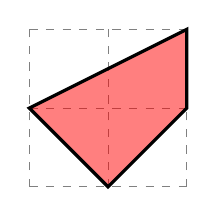
\begin{tikzpicture}
    \draw[gray, dashed] (0,0) grid (2,2);
    \draw[very thick, fill={red}, fill opacity=0.5] (0,1)--(1,0)--(2,1)--(2,2)--cycle;
  \end{tikzpicture}
  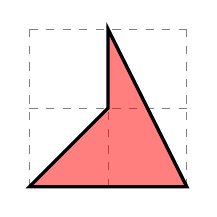
\begin{tikzpicture}
    \draw[gray, dashed] (0,0) grid (2,2);
    \draw[very thick, fill={red}, fill opacity=0.5] (0,0)--(2,0)--(1,2)--(1,1)--cycle;
  \end{tikzpicture}
  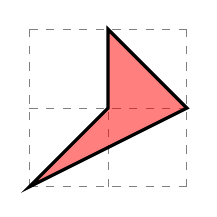
\begin{tikzpicture}
    \draw[gray, dashed] (0,0) grid (2,2);
    \draw[very thick, fill={red}, fill opacity=0.5] (0,0)--(2,1)--(1,2)--(1,1)--cycle;
  \end{tikzpicture}
  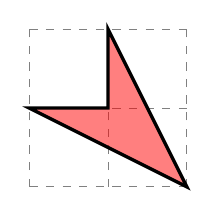
\begin{tikzpicture}
    \draw[gray, dashed] (0,0) grid (2,2);
    \draw[very thick, fill={red}, fill opacity=0.5] (0,1)--(2,0)--(1,2)--(1,1)--cycle;
  \end{tikzpicture}
  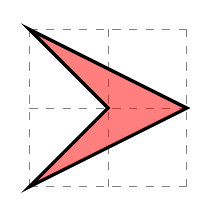
\begin{tikzpicture}
    \draw[gray, dashed] (0,0) grid (2,2);
    \draw[very thick, fill={red}, fill opacity=0.5] (0,0)--(1,1)--(0,2)--(2,1)--cycle;
  \end{tikzpicture}
  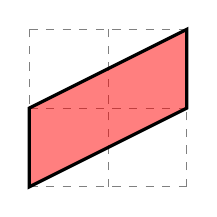
\begin{tikzpicture}
    \draw[gray, dashed] (0,0) grid (2,2);
    \draw[very thick, fill={red}, fill opacity=0.5] (0,0)--(0,1)--(2,2)--(2,1)--cycle;
  \end{tikzpicture}
  \caption{
    An example showing that $a_3(2) \geq 8$ and $a_4(2) \geq 14$.
  }
\end{figure}
\begin{question}
  What is $a_k(n)$?
\end{question}
\begin{related}
  \item For a fixed $n$, what is the value of $k$ such that $a_k(n)$ is
    maximized?
  \item Here two polygons are considered equivalent if they are congruent. What
  if two polygons are considered equivalent if they are similar?
  If they are the same under dihedral action?
  If they are the same over linear transformation? (e.g. stretching/skewing)
  \item What if concave polygons are excluded?
  \item What if this is done on an $n \times m$ grid?
  \item What if we don't deduplicate based on congruence?
  \item What if this is done on a hypercube or a triangular grid?
\end{related}

\end{document}
